\begin{figure}[!ht]
\captionsetup{belowskip=-1pt}
\begin{center}
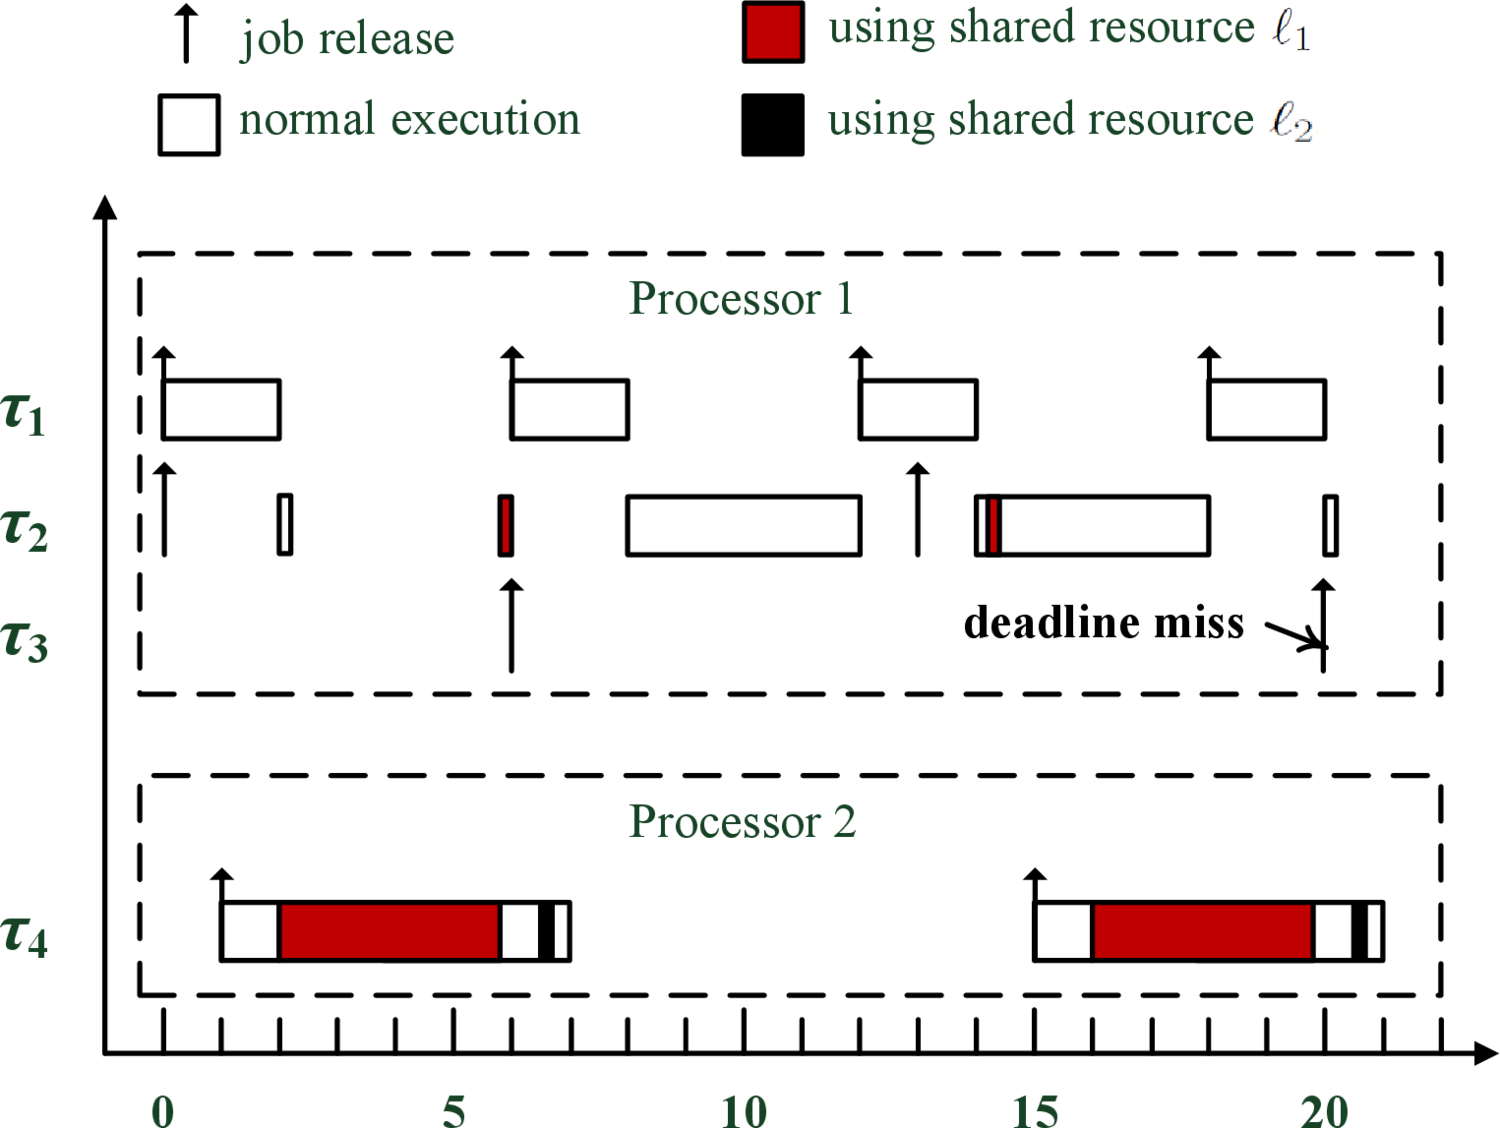
\includegraphics[width=12cm]{Counterexample}
\caption{An example schedule in which the first job of $\tau_3$ misses its deadline. 
\iffalse
The first job of $T_2$, denoted by $J_{2,1}$, releases at time $t=0$ and is scheduled at time $t=2$ when the first job of $T_1$ finishes.
At time $t=2+\varepsilon$, $J_{2,1}$ requests a shared resource $\res_1$ and incurs remote blocking (self-suspension) because $\res_1$ has been locked by $T_4$ at time $t=2$.
$J_{2,1}$ gets access to $\res_1$ until time $t=6-\varepsilon$. 
At time $t=6$, $J_{2,1}$ release $\res_1$ and is preempted by the second job of $T_1$, meanwhile, a job of $T_3$ releases. 
$J_{2,1}$ finishes at time $t=12$, and the second job of $T_2$, denoted by $J_{2,2}$, releases at time $t=13$. 
$J_{2,2}$ is scheduled at time $t=8$. 
It gets access to $\res_1$ at time $t=14+\varepsilon$ without incurring remote blocking (self-suspension), and it is always executing during $t \in [14,18)$.
Then, the forth job of $T_1$ releases, and it is executing during $t \in [20,22)$.
At time $t=22$, $J_{2,2}$ resumes, and the job of $T_3$ misses its deadline.
\fi
}
\label{fig:counterexample}
\end{center}
\end{figure}
